\section{Architecture and Design}\label{sec:archdesign}

\subsection{Architecture}
\begin{framed}
3. Use your design methodology found in 1. to describe a SysML/UML model of your system in terms of structure and behavior. Make a suggestion for alternative HW/SW architectures. Decide on which parts of the functionality should be mapped to hardware components and software processes.
\end{framed}

The overall structure of the system can be seen in the BDD in figure \ref{fig:bdd}. Here it can be seen, that the system should consist of three parts: \emph{User Interface}, \emph{Generation Generator}, and \emph{Simulator}. Each of the blocks has its own responsibility. \emph{User Interface} is responsible for getting the input from and to the user, e.g. the start generation and the final generation and fitness. \emph{Generation Generator} is responsible for generating the new generation using the genetic algorithm. \emph{Simulator} is responsible for calculating the fintness, i.e. the Rosenbrock function.

\begin{figure}[htbp]
\begin{centering}
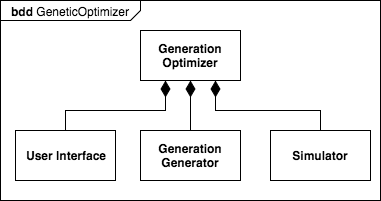
\includegraphics[width=0.7\linewidth]{../diagrams/bdd.png}
\caption{BDD of the system.}
\label{fig:bdd}
\end{centering}
\end{figure}





NOTE: waits in rosenbrock to reduce resources used


\subsection{Design}

\begin{framed}
4. Design the software and apply design patterns that are suitable for your project, and motivate the choice of the used patterns. Use the Two-Part Architecture Model if relevant for the problem. Use the abstract OS package for the ZYBO board
\end{framed}